\documentclass[12pt]{beamer}

\usepackage[T2A]{fontenc}
\usepackage[utf8]{inputenc}
\usepackage[russian,english]{babel}
\usepackage{subfig}
\usepackage[noend]{algorithm,algpseudocode}
\usepackage{amsmath}

\usepackage{booktabs}
\usepackage[scale=2]{ccicons}

\usepackage{pgfplots}
\usepgfplotslibrary{dateplot}

\usepackage{xspace}
\newcommand{\TODO}[1]{\textbf{\textcolor{red}{TODO: #1}}}


\algblockdefx{MRepeat}{EndRepeat}{\textbf{repeat}}{}
\algnotext{EndRepeat}

\algrenewcommand\alglinenumber[1]{\footnotesize #1}
\DeclareMathOperator{\rank}{rank}
\DeclareMathOperator{\sign}{sign}

\newcounter{mycounter}

\newcommand{\myparagraph}{\stepcounter{mycounter}\paragraph{\arabic{mycounter}}}

\title{Лекция 9}
\subtitle{Метод опорных векторов.}

\begin{document}	

\section{Разбор летучки}

\frame{\titlepage}

\begin{frame}{Постановка задачи}
	$X = \mathbb{R}^n$, ${Y = \left\{ -1, + 1\right\}}$\\
	${X^l = (x_i, y_i)_{i = 1}^l}$ -- обучающая выборка\\
  \bigbreak
	Линейный классификатор:\\
	$a(\mathbf{x}, \mathbf{w}) = sign(\langle \mathbf{w}, \mathbf{x}\rangle - w_0)$\\	
	\bigbreak
	Найти:\\
	$(n-1)$-мерную гиперплоскость, которая разделяет данные как можно лучше.
\end{frame}

\section{Линейно разделимая выборка}

\begin{frame}{Линейно разделимая выборка}
	\begin{figure}[htbp]
	  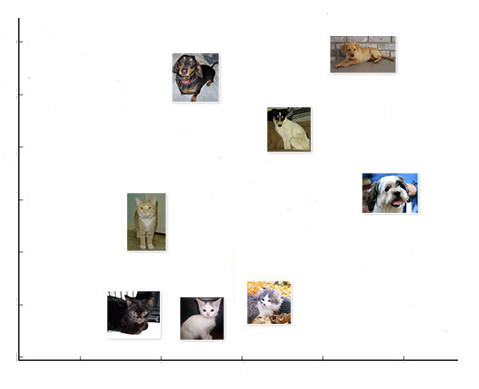
\includegraphics[height=190pt, keepaspectratio = true]{images/linearly_separable1}   
	\end{figure}
\end{frame}

\begin{frame}{Линейно неразделимая выборка}
	\begin{figure}[htbp]
	  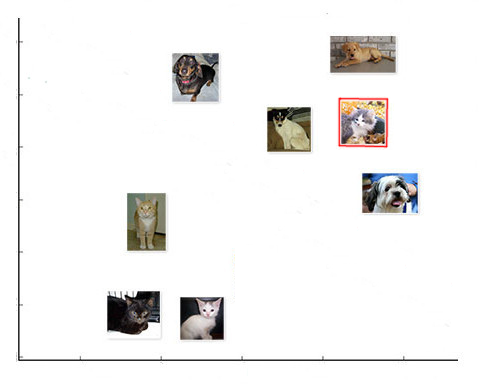
\includegraphics[height=190pt, keepaspectratio = true]{images/linearly_unseparable}   
	\end{figure}
\end{frame}

\begin{frame}{Линейно разделимая выборка}
	Выборка линейно разделима, если отступ на каждом объекте положителен.\\
	\bigbreak
	$\exists \mathbf{w}, w_0 : M_i(\mathbf{w}, w_0) = y_i  (\langle \mathbf{w}, \mathbf{x_i} \rangle - w_0) > 0, \qquad i=1, \dots , l$\\
	\bigbreak
	\pause
  Нормировка: $\min\limits_{i = 1, \dots , l} M_i(\mathbf{w}, w_0) = 1$\\
\end{frame}

\begin{frame}{Разделяющая гиперплоскость}
  \centering
  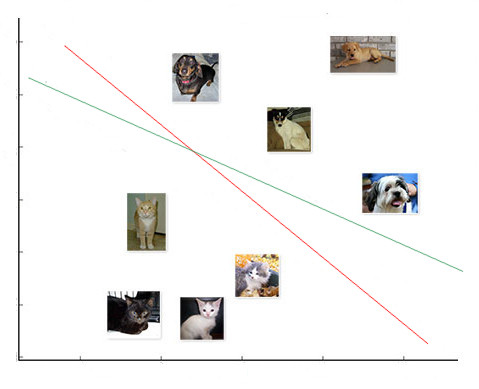
\includegraphics[width=0.9 \textwidth, keepaspectratio]{images/catdog}
\end{frame}

\begin{frame}{Максимизиция отступа}
	\alert{Идея}: Будем искать такую разделяющую поверхность, которая обеспечивает разделяющую полосу максимальной ширины.\\
\end{frame}

\begin{frame}{Пример}
  \centering
  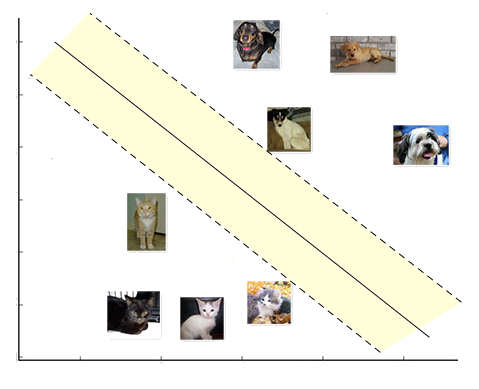
\includegraphics[width=0.9 \textwidth, keepaspectratio]{images/margin}
\end{frame}

\begin{frame}{Пример}
  \centering
  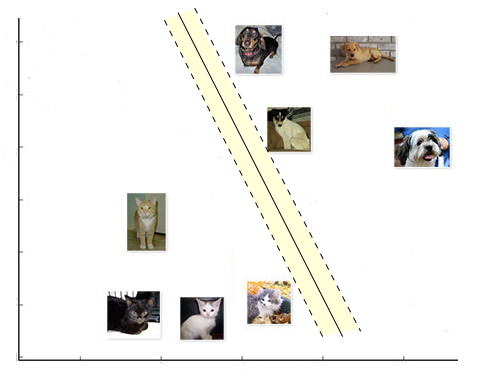
\includegraphics[width=0.9 \textwidth, keepaspectratio]{images/margin1}
\end{frame}

\section{Опорная гиперплоскость}

\begin{frame}{Опорная гиперплоскость}
	Гиперплоскость называется опорной для множества точек
	$X$, если все точки из $X$ лежат по одну сторону от этой гиперплоскости.\\\bigbreak
	${a(\mathbf{x},\mathbf{w}, w_0) = \langle \mathbf{x}, \mathbf{w}\rangle - w_0 = 0}$\\
	\bigbreak
	\onslide<1>{
    	Как посчитать расстояние от точки до гиперплоскости?
  }
  \onslide<2>{
    Расстояние от точки до гиперплоскости = $\frac{\vert a(\mathbf{x},\mathbf{w}, w_0) \vert}{\Vert \mathbf{w} \Vert}$
  }
\end{frame}

\begin{frame}{Максимизиция отступа}
	\alert{Идея}: Максимизировать отступ между двумя параллельными опорными плоскостями, а затем провести параллельную им плоскость на равных расстояниях.\\
\end{frame}

\begin{frame}{Оптимальная разделяющая гиперплоскость}
	\onslide<1>{
    	Как выглядит разделяющая полоса?\\
	}
	\onslide<2>{
    	Разделяющая полоса: $\left\{\mathbf{x}: -1 \leq \langle \mathbf{w}, \mathbf{x}\rangle - w_0 \leq 1\right\}$
	}
	\begin{figure}[htbp]
	  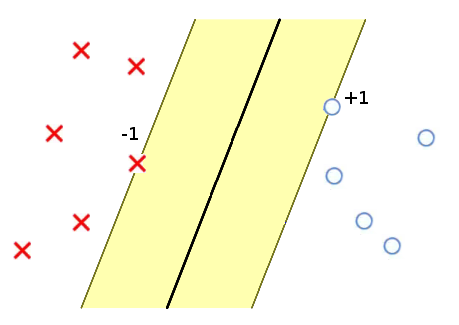
\includegraphics[height=100pt, keepaspectratio = true]{images/linearly_separable3}   
	\end{figure}
\end{frame}

\begin{frame}{Оптимальная разделяющая гиперплоскость}
	Разделяющая полоса: $\left\{\mathbf{x}: -1 \leq \langle \mathbf{w}, \mathbf{x}\rangle - w_0 \leq 1\right\}$\\
	\onslide<1>{
  	  Ширина разделяющей полосы?\\
  	  }
  	\onslide<2>{
    	Ширина разделяющей полосы: $\frac{\langle \mathbf{x_{+}}, \mathbf{w} \rangle + \langle \mathbf{x_{-}}, \mathbf{w} \rangle}{\Vert \mathbf{w} \Vert} = \frac{2}{\Vert \mathbf{w} \Vert} \rightarrow \max$\\
  	}
	\begin{figure}[htbp]
	  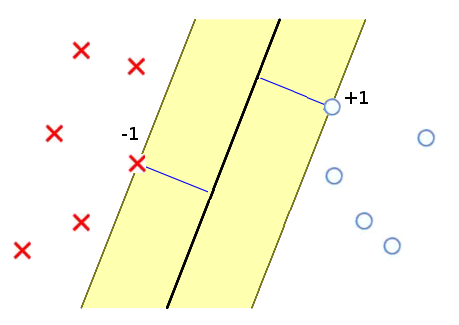
\includegraphics[height=100pt, keepaspectratio = true]{images/linearly_separable2}   
	\end{figure}
\end{frame}

\begin{frame}{Оптимальная разделяющая гиперплоскость}
	Линейно разделимая выборка:\\
	$\begin{cases}
		{\frac{1}{2} \Vert \mathbf{w} \Vert^2 \rightarrow \min\limits_{\mathbf{w}}}\\
		M_i(\mathbf{w}, w_0) \geq 1   \qquad i = 1, \dots, l
	\end{cases}$\\
	\pause
	\bigbreak
	Линейно неразделимая выборка -- надо ослабить имеющиеся условия.\\
	$\begin{cases}
		{\frac{1}{2}\Vert \mathbf{w} \Vert^2 + \textcolor{orange}{C \sum\limits_{i=1}^l \xi_i} \rightarrow \min\limits_{\mathbf{w}, \xi}}\\
		M_i(\mathbf{w}, w_0) \geq 1 - \textcolor{orange}{\xi_i} \qquad i = 1, \dots, l\\
		\textcolor{orange}{\xi_i \geq 0} \qquad i = 1, \dots, l
	\end{cases}$\\
\end{frame}

\begin{frame}{Оптимальная разделяющая гиперплоскость}
	$\begin{cases}
		\xi_i \geq 1 - M_i(\mathbf{w}, w_0) \\
		\xi_i \geq 0
	\end{cases} \Rightarrow \xi_i = 1 - M_i(\mathbf{w}, w_0) $\\
	\begin{figure}[htbp]
	  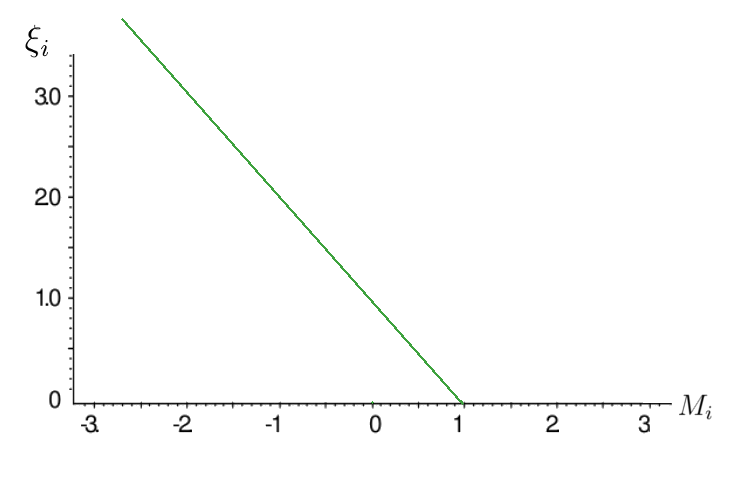
\includegraphics[height=100pt, keepaspectratio = true]{images/xi}   
  \end{figure}
\end{frame}

\begin{frame}{Задача безусловной минимизации}
	$\begin{cases}
		{\frac{1}{2}\Vert \mathbf{w} \Vert^2 + C \sum\limits_{i=1}^l \xi_i \rightarrow \min\limits_{\mathbf{w}, \xi}}\\
		\xi_i = 1 - M_i(\mathbf{w}, w_0)
	\end{cases}$\\
	\bigbreak
	\pause
	Задача безусловной минимизации:\\
	$ C \sum\limits_{i=1}^l (1 - M_i(\mathbf{w}, w_0)) + \frac{1}{2}\Vert \mathbf{w} \Vert^2 \rightarrow \min\limits_{\mathbf{w}}$
\end{frame}

\begin{frame}{Минимизация эмпирического риска}
	${Q(\mathbf{w}) = \sum\limits_{i=1}^l \left[ M_i(\mathbf{w}, w_0) < 0 \right] \leq\sum\limits_{i=1}^l \mathcal{L}(M_i(\mathbf{w}, w_0)) \rightarrow \min\limits_{\mathbf{w}} }$\\\vspace{3mm}
	\bigbreak
	\pause
	Штраф за увеличение нормы вектора весов:\\
	$Q_{\tau} = Q + \frac{\tau}{2}\Vert \mathbf{w} \Vert^2 \rightarrow \min\limits_{\mathbf{w}}$\\
	\bigbreak
	\pause
	Метод опорных векторов:\\
	$ C\sum\limits_{i=1}^l (1 - M_i(\mathbf{w}, w_0)) + \frac{1}{2}\Vert \mathbf{w} \Vert^2 \rightarrow \min\limits_{\mathbf{w}}$
\end{frame}

\begin{frame}{Примеры $\mathcal{L}$}
	\begin{figure}[htbp]
	  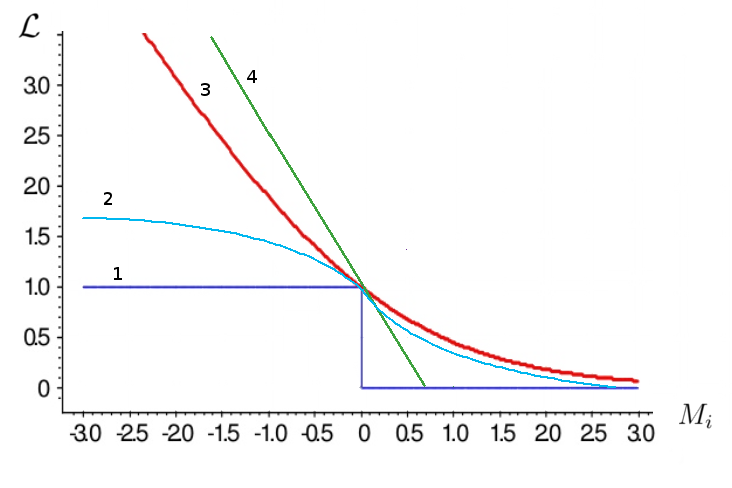
\includegraphics[height=160pt, keepaspectratio = true]{images/l}
	\end{figure}
	\begin{enumerate}
		\item $\left[M_i(\mathbf{w}, w_0) < 0 \right]$
		\item $L(M) = \log_2(1+e^{-M})$ -- логарифмическая
		\item $S(M) = 2(1+e^M)^{-1}$ -- сигмоидная
		\item $V(M) = (1-M)_+$ -- кусочно-линейная
	\end{enumerate}
\end{frame}

\begin{frame}{Вопрос}
	$ \sum\limits_{i=1}^l (1 - M_i(\mathbf{w}, w_0)) + \frac{1}{2C}\Vert \mathbf{w} \Vert^2 \rightarrow \min\limits_{\mathbf{w}}$\\
	\bigbreak
	На что влияет параметр $C$?
\end{frame}

{\foot{Пример из Python scikit-learn: http://scikit-learn.org/dev}
\begin{frame}{Выбор параметра $C$}
	\begin{figure}[htbp]
		\begin{minipage}{.5\textwidth}
		  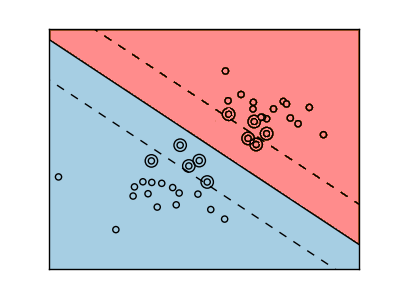
\includegraphics[height=120pt, keepaspectratio = true]{images/svm_reg} \\
			\centering Маленький $C$\\ Сильная регуляризация\\
	  \end{minipage}%
	  \begin{minipage}{.5\textwidth}
			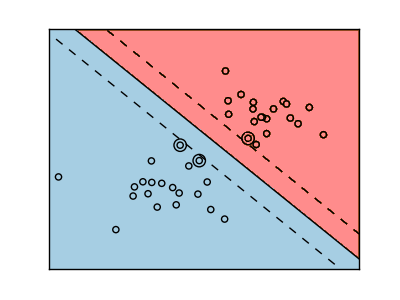
\includegraphics[height=120pt, keepaspectratio = true]{images/svm_non_reg}   \\
		  \centering Большой $C$\\ Слабая регуляризация\\
		\end{minipage}%
	\end{figure}
\end{frame}
}

{\foot{Функция Лагранжа}
\begin{frame}{Условие Каруша-Куна-Такера}
	$\begin{cases}
		f(x) \rightarrow \min\\
		g_i(x) \leq 0 , i = 1, \dots, m\\
		h_j(x) = 0 , j = 1, \dots, k\\
	\end{cases}$\\
	\bigbreak
	\pause
	Двойственная задача:\\
	$\begin{cases}
		\mathcal{L}(x; \mu, \alpha) = f(x) + \sum\limits_{i = 1}^m \mu_ig_i(x) + \sum\limits_{j = 1}^k \alpha_jh_j(x)\\
		\frac{\partial \mathcal{L}}{\partial x} = 0\\
		g_i(x) \leq 0 , h_j(x) = 0\\
		\mu_i \geq 0\\
		\mu_ig_i(x) = 0
	\end{cases}$\\
\end{frame}
}

\begin{frame}{Двойственная задача SVM}
	$\begin{cases}
		{\frac{1}{2}\Vert \mathbf{w} \Vert^2 + C \sum\limits_{i=1}^l \xi_i \rightarrow \min\limits_{\mathbf{w}, \xi}}\\
		M_i(\mathbf{w}, w_0) \geq 1 - \xi_i\\
		\xi_i \geq 0
	\end{cases}$\\
	\bigbreak
	\pause
	Двойственная задача:\\
	$\begin{cases}
		\mathcal{L} = \frac{1}{2} \Vert \mathbf{w} \Vert^2 - \sum\limits_{i = 1}^l \alpha_i (M_i(\mathbf{w}, w_0) - 1) - \sum\limits_{i = 1}^l \xi_i (\alpha_i + \mu_i - C)\\
		\xi_i \geq 0, \qquad  \alpha_i \geq 0,  \qquad  \mu_i \geq 0\\
		\alpha_i = 0$ либо $M_i(\mathbf{w}, w_0) = 1 - \xi_i ,  \qquad i = 1, \dots, l\\
		\mu_i = 0 $ либо $\xi_i = 0, \qquad i = 1, \dots, l
	\end{cases}$
\end{frame}

\begin{frame}{Двойственная задача SVM}
	$\mathcal{L}(\mathbf{w}, w_0, \xi) = \frac{1}{2} \Vert \mathbf{w} \Vert^2 - \sum\limits_{i = 1}^l \alpha_i (M_i(\mathbf{w}, w_0) - 1) - \sum\limits_{i = 1}^l \xi_i (\alpha_i + \mu_i -C)$\\
	\bigbreak
	\pause
	$\frac{\partial \mathcal{L}}{\partial \mathbf{w}}  = \mathbf{w} - \sum\limits_{i=1}^l \alpha_iy_i\mathbf{x_i} = 0 $ \hspace{5mm} $\Rightarrow \mathbf{w} = \sum\limits_{i=1}^l \alpha_iy_i\mathbf{x_i} = 0$\\
	\pause
	$\frac{\partial \mathcal{L}}{\partial w_0} = - \sum\limits_{i=1}^l \alpha_iy_i = 0$ \hspace{12mm} $\Rightarrow \sum\limits_{i=1}^l \alpha_iy_i = 0$\\
	\pause
	$\frac{\partial \mathcal{L}}{\partial \xi_i} = -\alpha_i - \mu_i + C = 0$ \hspace{6mm}  $\Rightarrow \mu_i + \alpha_i = C$\\
\end{frame}

\begin{frame}{Двойственная задача SVM}
	$\begin{cases}
	  -\mathcal{L}(\alpha) = - \sum\limits_{i = 1}^l \alpha_i  + \frac{1}{2} \sum\limits_{i = 1}^l\sum\limits_{j = 1}^l \alpha_i \alpha_j y_iy_j \langle \mathbf{x_i}, \mathbf{x_j} \rangle \rightarrow \min\limits_{\alpha}\\
	0 \leq \alpha_i \leq C\\
	\sum\limits_{i=1}^l \alpha_iy_i = 0
	\end{cases}$\\
\end{frame}

\begin{frame}{Двойственная задача SVM}
	Решение исходной задачи выражается через решение двойственной:\\
	$\begin{cases}
	\mathbf{w} = \sum\limits_{i = 1}^l \alpha_iy_i\mathbf{x_i}\\
	w_0 = \langle \mathbf{w}, \mathbf{x_i} \rangle - y_i
	\end{cases}$\\
	\bigbreak
	\pause
	Линейный классификатор:\\
	$a(\mathbf{x}) = \sign(\sum\limits_{i=1}^l \alpha_iy_i \langle \mathbf{x_i}, \mathbf{x} \rangle - w_0)$
\end{frame}

\begin{frame}{Понятие опорного вектора}
	\begin{itemize}
		\item[--] $\alpha_i = 0$, $M_i \geq 1$ -- неинформативные объекты
		\item[--] $0 < \alpha_i < C$, $M_i = 1$ -- опорные объекты
		\item[--] $\alpha_i = C$, $M_i < 1$ -- опорные объекты-нарушители
	\end{itemize}
	
	\begin{figure}[htbp]
	  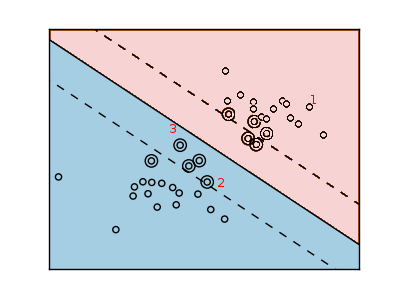
\includegraphics[height=100pt, keepaspectratio = true]{images/classification}   
	\end{figure}
\end{frame}

\section{Kernel trick}

\begin{frame}{Kernel trick}
	$\langle \mathbf{x_i}, \mathbf{x} \rangle \rightarrow K(\mathbf{x_i}, \mathbf{x})$\\
	\bigbreak
	$\psi: X \rightarrow H$, \qquad $H$ - Гильбертово пространство\\
	$K(\mathbf{x_i}, \mathbf{x}) = \langle \mathbf{\psi(x_i)}, \mathbf{\psi(x)} \rangle_H$
	\begin{itemize}
		\item[--] $K(\mathbf{x_i}, \mathbf{x}) = K(\mathbf{x}, \mathbf{x_i})$
		\item[--] неотрицательно определена
	\end{itemize}
\end{frame}

\begin{frame}{Переход к более высокой размерности}
	\begin{figure}[htbp]
		\begin{minipage}{.5\textwidth}
		  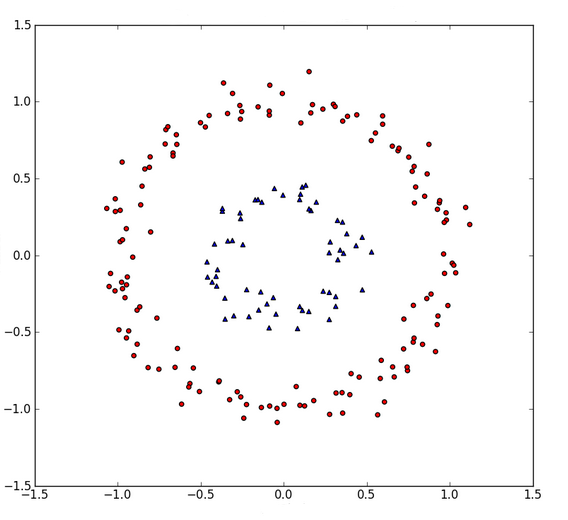
\includegraphics[height=120pt, keepaspectratio = true]{images/data-r2} \\
			\centering Данные в $\mathbb{R}^2$
	  \end{minipage}%
	  \begin{minipage}{.5\textwidth}
			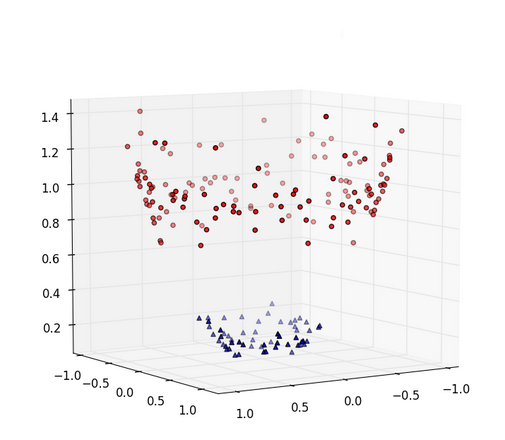
\includegraphics[height=120pt, keepaspectratio = true]{images/data-r3}   \\
			\centering Данные в $\mathbb{R}^3$
		\end{minipage}%
	
	\end{figure}
\end{frame}

\begin{frame}{Переход к более высокой размерности}
	\begin{figure}[htbp]
		\begin{minipage}{.5\textwidth}
		  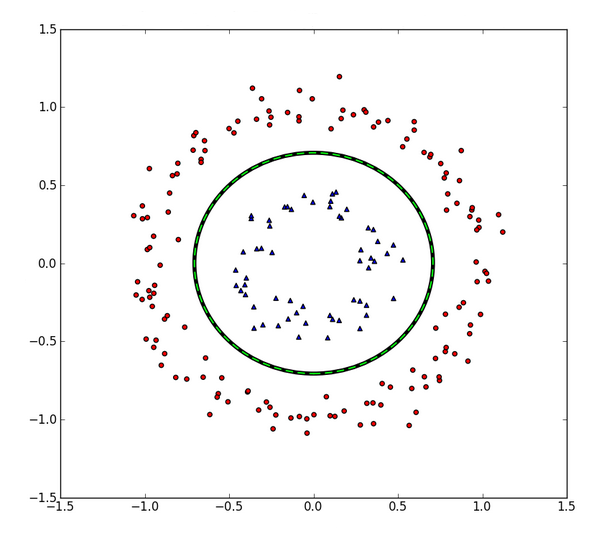
\includegraphics[height=120pt, keepaspectratio = true]{images/data-r2-1} \\
			\centering Данные в $\mathbb{R}^2$
	    \end{minipage}%
	    \begin{minipage}{.5\textwidth}
			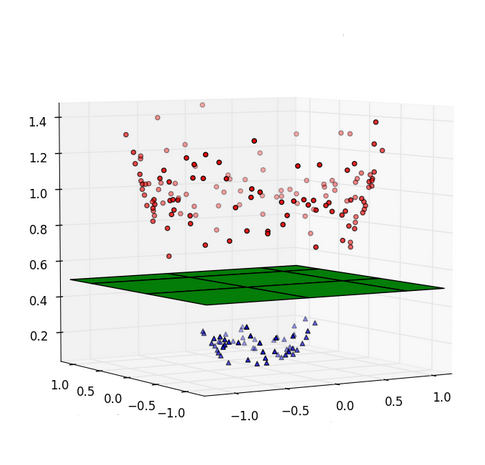
\includegraphics[height=120pt, keepaspectratio = true]{images/data-r3-1}   \\
			\centering Данные в $\mathbb{R}^3$
		\end{minipage}%
	
	\end{figure}
\end{frame}

{\foot{Пример из Python scikit-learn: http://scikit-learn.org/dev}
\begin{frame}{Примеры ядер}
	\begin{figure}[htbp]
		\begin{minipage}{.3\textwidth}
		  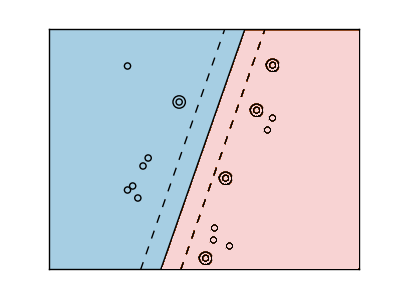
\includegraphics[height=70pt, keepaspectratio = true]{images/linear} \\
		  \centering Линейное\\$\langle x, x'\rangle$
	    \end{minipage}%
	    \begin{minipage}{.3\textwidth}
			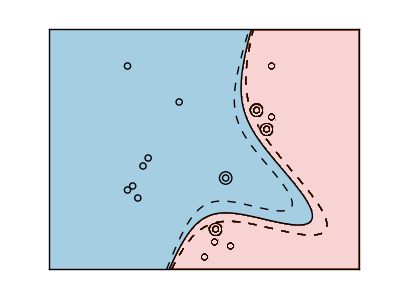
\includegraphics[height=70pt, keepaspectratio = true]{images/poly}   \\
			\centering Полиномиальное\\$(\langle x, x'\rangle + 1)^3$
		\end{minipage}%
	    \begin{minipage}{.3\textwidth}
			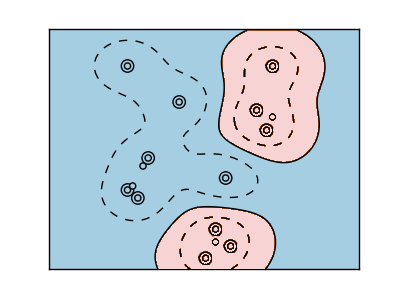
\includegraphics[height=70pt, keepaspectratio = true]{images/gauss}   \\
			\centering Гауссовское\\$exp(-\beta \Vert x - x'\Vert^2 )$
		\end{minipage}%
	
	\end{figure}
\end{frame}
}

\begin{frame}{Примеры ядер}
	\begin{figure}[htbp]
	  \centering Гауссовское\\$exp(-\beta \Vert x - x'\Vert^2 )$\\
	  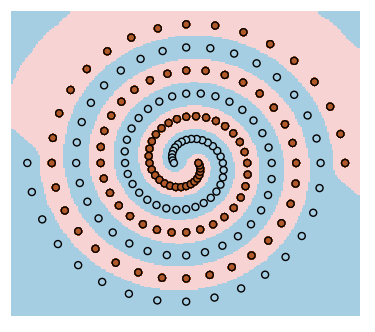
\includegraphics[height=160pt, keepaspectratio = true]{images/svm_spiral}
	\end{figure}
\end{frame}

\begin{frame}{Конструктивные методы получения ядер}
	\begin{itemize}
		\item[--] $K(\mathbf{x_i}, \mathbf{x}) = \langle \mathbf{x_i}, \mathbf{x} \rangle$
		\item[--] $K(\mathbf{x_i}, \mathbf{x}) = const$
		\item[--] $K(\mathbf{x_i}, \mathbf{x}) = K_1(\mathbf{x_i}, \mathbf{x}) K_2(\mathbf{x_i}, \mathbf{x})$
		\item[--] $K(\mathbf{x_i}, \mathbf{x}) = \alpha_1 K_1(\mathbf{x_i}, \mathbf{x}) + \alpha_2 K_2(\mathbf{x_i}, \mathbf{x})$ при  $\alpha_1, \alpha_2 > 0$
		\item[--] $\forall \psi: X \rightarrow \mathbb{R}$ \hspace{5mm}$K(\mathbf{x_i}, \mathbf{x}) = \psi(\mathbf{x_i}) \psi(\mathbf{x})$
		\item[--] $\forall \phi: X \rightarrow X$ \hspace{5mm}$K(\mathbf{x_i}, \mathbf{x}) = K_0(\phi(\mathbf{x_i}),  \phi(\mathbf{x}))$
	\end{itemize}
\end{frame}

\begin{frame}{Примеры ядер}
	\begin{itemize}
		\item[--] $K(\mathbf{x_i}, \mathbf{x}) = \langle \mathbf{x_i}, \mathbf{x} \rangle^d$
		\item[--] $K(\mathbf{x_i}, \mathbf{x}) = (\langle \mathbf{x_i}, \mathbf{x} \rangle + 1)^d$
		\item[--] $K(\mathbf{x_i}, \mathbf{x}) = \sigma (\langle \mathbf{x_i}, \mathbf{x} \rangle)$\\
		  Двуслойная нейросеть с функцией активации $\sigma$
		\item[--] $K(\mathbf{x_i}, \mathbf{x}) = th (k_0 + k_1 \langle \mathbf{x_i}, \mathbf{x} \rangle), \qquad k_0, k_1 \geq 0$
		\item[--] $K(\mathbf{x_i}, \mathbf{x}) = \exp (-\beta \| \mathbf{x} - \mathbf{x_i} \|^2 )$
	\end{itemize}
\end{frame}

\begin{frame}{Достоинства и недостатки}
	\begin{itemize}[<+->]
		\item[+] Задача имеет единственное решение
		\item[+] Число опорных векторов определяется автоматически
	  \bigbreak
	
		\item[--] Неустойчивость к шуму
		\item[--] Нет общих подходов к оптимизации ядра под задачу
		\item[--] Подбор константы C
	\end{itemize}
\end{frame}

\begin{frame}{SVM как двуслойная нейросеть}
  \centering
  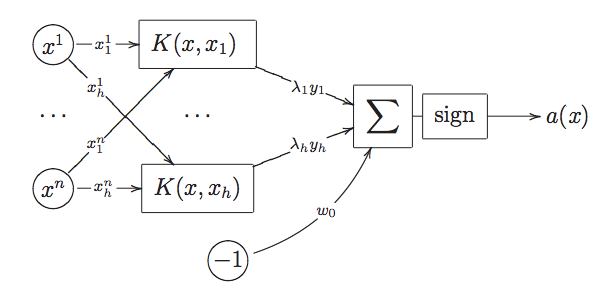
\includegraphics[width=\textwidth, keepaspectratio]{images/svm_nn}\\
  \bigbreak
  $h$ -- количество опорных объектов
\end{frame}

\begin{frame}[standout]
  Вопросы?
\end{frame}

\appendix

\begin{frame}\frametitle{Что почитать по этой лекции}
  \begin{itemize}
    \item T. Hastie, R. Tibshirani "The Elements of Statistical Learning" Chapter 12
    \item Andrew Ng \href{http://cs229.stanford.edu/notes/cs229-notes3.pdf}{CS229 Lecture notes}
    \item M. Morhi, A. Rostamizadeh, A. Talwalkar "Foundations of Machine Learning"
  \end{itemize}
\end{frame}

\begin{frame}{На следующей лекции}
	\begin{itemize}
    	\item[--] Линейная регрессия
    \item[--] Многомерная регрессия
    \item[--] Проблема мультиколлинеарности
    \item[--] Сингулярное разложение
    \item[--] Гребневая регрессия
    \item[--] Lasso    
	\end{itemize}
\end{frame}

\end{document}
